\chapter{Ligand Field Theory and Colour}\label{ch:b2:ligand-field}

Ruby is red and emerald is green, yet both owe their colour to the same ion,
\ce{Cr^3+}, a few of which replace aluminium in corundum, \ce{Al2O3}, or in
beryl. Copper sulfate crystals are deep blue, but the powder left after
heating them is white. In each case the colour comes from electrons jumping
between d orbitals whose energies the surrounding atoms have pulled apart ---
by an amount that depends on which atoms surround the ion and how. This
chapter computes that splitting, first with point charges, then with \omterm{def:b2:diatomic-mos:lcao}{molecular
orbitals}; it explains colours, magnetism, and the \omterm{def:b2:coordination-complexes:electron-count}{18-electron rule} of the
previous chapter.

\begin{recall}
\Cref{ch:b2:coordination-complexes}: $d^n$ configurations, geometries, electron
counts. \Cref{ch:b2:atomic-orbitals}: the shapes of the five d orbitals.
\Cref{ch:b2:fragment-orbitals}: \omterm{def:b2:fragment-orbitals:fragment}{fragment orbitals}. The Year 1 volume: absorbance,
complementary colours, unpaired electrons, Hund's rule.
\end{recall}

\begin{omfigure}
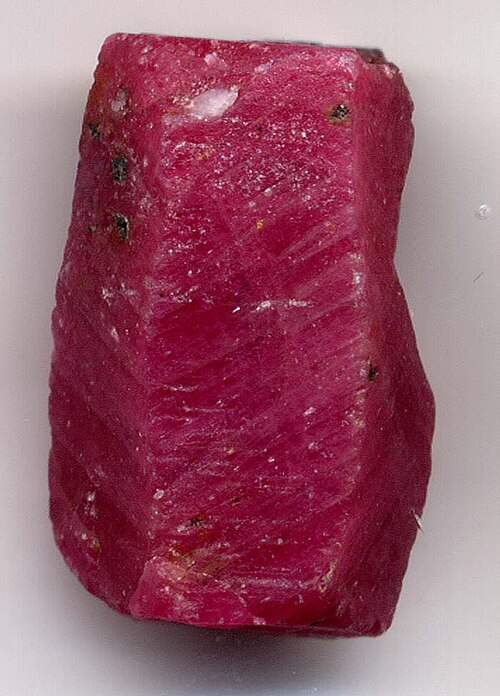
\includegraphics[height=3.6cm]{images/book3/ruby.jpg}\hspace{0.6cm}%
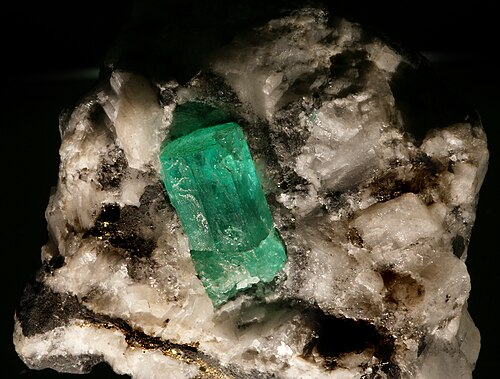
\includegraphics[height=3.6cm]{images/book3/emerald.jpg}\hspace{0.6cm}%
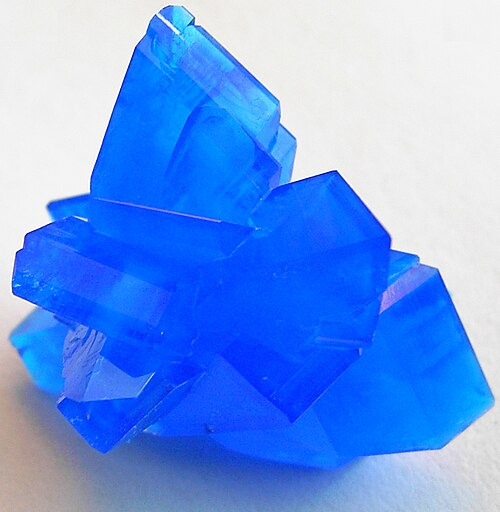
\includegraphics[height=3.6cm]{images/book3/copper-sulfate.jpg}

{\small A ruby crystal (public domain); an emerald in its rock (Didier Descouens,
CC BY-SA 3.0); crystals of copper(II) sulfate pentahydrate (Stephanb, CC BY-SA
3.0). Wikimedia Commons. Chromium(III) colours the first two, the aqua complex of
copper(II) the third.}
\end{omfigure}

\section{The crystal-field model}

\begin{definition}[Crystal field]\label{def:b2:ligand-field:crystal-field}
The \emph{crystal-field model}\index{crystal-field model} treats the ligands of a
complex as negative point charges (or the negative ends of dipoles) around the metal
ion, and computes how they change the energies of its d orbitals. In an octahedral
field, the d orbitals split into two sets separated by the \emph{crystal-field
splitting}\index{crystal-field splitting} $\Delta_o$.
\end{definition}

Place the six ligands on the axes. The $\mathrm d_{z^2}$ and $\mathrm d_{x^2-y^2}$
orbitals point their lobes straight at ligands: an electron in them is repelled more
and they rise. The $\mathrm d_{xy}$, $\mathrm d_{xz}$, $\mathrm d_{yz}$ orbitals point between
the ligands and rise less. The first pair is called $e_g$, the second set of three
$t_{2g}$ (names from group theory, in the Year 3 volume).

\begin{omfigure}
\begin{tikzpicture}[font=\small]
  \begin{scope}
    \pic at (0,0) {omdx2y2};
    \foreach \p in {(1.25,0),(-1.25,0),(0,1.25),(0,-1.25)} \node[circle, fill=black!70, inner sep=2.2pt] at \p {};
    \node at (0,-1.75) {$\mathrm d_{x^2-y^2}$: lobes at the ligands};
  \end{scope}
  \begin{scope}[xshift=5.5cm]
    \pic at (0,0) {omdxy};
    \foreach \p in {(1.25,0),(-1.25,0),(0,1.25),(0,-1.25)} \node[circle, fill=black!70, inner sep=2.2pt] at \p {};
    \node at (0,-1.75) {$\mathrm d_{xy}$: lobes between them};
  \end{scope}
\end{tikzpicture}

{\small Two d orbitals among the four ligands of the $xy$ plane of an octahedron
(black dots). The lobes of $\mathrm d_{x^2-y^2}$ point at the ligands, those of
$\mathrm d_{xy}$ between them.}
\end{omfigure}

\begin{theorem}[Barycentre]\label{thm:b2:ligand-field:barycentre}
In an octahedral field, measured from the average energy of the d orbitals, the
$e_g$ pair lies at $+0.6\Delta_o$ and the $t_{2g}$ set at $-0.4\Delta_o$.
\end{theorem}

\begin{proof}
The field raises the average of the five d energies but does not change it by
splitting (the barycentre rule, admitted: the sum of the shifts of a full set of
orbitals is fixed by the total charge, not by its arrangement). With $e_g$ at $x$ and
$t_{2g}$ at $x - \Delta_o$, the condition $2x + 3(x - \Delta_o) = 0$ gives $x = 0.6\Delta_o$.
\end{proof}

\section{High spin and low spin}

\begin{definition}[Spin states]\label{def:b2:ligand-field:spin}
The \emph{pairing energy}\index{pairing energy} $P$ is the energy needed to put a second
electron into an occupied orbital rather than into an empty one of the same energy. A
complex is \emph{high spin}\index{high spin} when its electrons occupy the $e_g$ orbitals
before pairing in $t_{2g}$, \emph{low spin}\index{low spin} when they pair in $t_{2g}$
first.
\end{definition}

\begin{proposition}[Choice of the spin state]\label{prop:b2:ligand-field:spin-state}
For $d^4$ to $d^7$ octahedral ions, the complex is \omterm{def:b2:ligand-field:spin}{low spin} if $\Delta_o > P$ and \omterm{def:b2:ligand-field:spin}{high spin}
if $\Delta_o < P$. For $d^1$--$d^3$ and $d^8$--$d^{10}$ only one configuration exists.
\end{proposition}

\begin{proof}
From $d^3$ ($t_{2g}^3$), the fourth electron either enters $e_g$ (cost $\Delta_o$ above
$t_{2g}$) or pairs in $t_{2g}$ (cost $P$). The cheaper wins; the same comparison holds
for each electron up to $d^7$. For $d^1$--$d^3$ there is room in $t_{2g}$ without pairing;
for $d^8$--$d^{10}$, $t_{2g}$ is full and $e_g$ must be used anyway.
\end{proof}

\begin{definition}[Crystal-field stabilisation energy]\label{def:b2:ligand-field:cfse}
The \emph{crystal-field stabilisation energy}\index{crystal-field stabilisation
energy} (CFSE) of a configuration $t_{2g}^ae_g^b$ is $(-0.4a + 0.6b)\Delta_o$, the energy of
the d electrons relative to the barycentre (the pairing energies counted separately).
\end{definition}

\begin{proposition}[CFSE along the series]\label{prop:b2:ligand-field:cfse}
\omterm{def:b2:ligand-field:spin}{High spin}, the CFSE is $0$, $-0.4$, $-0.8$, $-1.2$, $-0.6$, $0$, $-0.4$, $-0.8$, $-1.2$,
$-0.6$, $0$ (in $\Delta_o$) for $d^0$ to $d^{10}$: it vanishes for $d^0$, $d^5$, $d^{10}$. \omterm{def:b2:ligand-field:spin}{Low
spin} it reaches $-2.4\Delta_o$ for $d^6$.
\end{proposition}

\begin{proof}
Fill the configurations and apply the definition; the values are those of the figure,
computed.
\end{proof}

\begin{omfigure}
\begin{tikzpicture}
\begin{axis}[width=0.55\linewidth, height=5cm, xmin=-0.5, xmax=10.5, ymin=-2.6, ymax=0.3,
  axis x line=bottom, axis y line=left, xlabel={$d^n$}, ylabel={CFSE ($\Delta_o$)},
  xtick={0,1,2,3,4,5,6,7,8,9,10}, tick label style={font=\small}, label style={font=\small}]
\addplot[omThm, thick, mark=*, mark size=1.3pt] table[x=n, y=high] {figdata/out/bachelor-2-ligand-field-a.dat};
\addplot[omDef, thick, dashed, mark=square*, mark size=1.3pt] table[x=n, y=low] {figdata/out/bachelor-2-ligand-field-a.dat};
\node[font=\scriptsize, omThm, anchor=west] at (axis cs:5.4,0.0) {high spin};
\node[font=\scriptsize, omDef, anchor=west] at (axis cs:6.6,-2.2) {low spin};
\end{axis}
\end{tikzpicture}\hfill
\begin{tikzpicture}[font=\small]
  \pic (t) at (0,0) {omlevel={ud}{0.5}}; \pic at (0.6,0) {omlevel={u}{0.5}}; \pic at (1.2,0) {omlevel={u}{0.5}};
  \pic at (0.3,1.6) {omlevel={u}{0.5}}; \pic at (0.9,1.6) {omlevel={u}{0.5}};
  \node at (0.6,-0.8) {high spin $d^6$};
  \node[font=\scriptsize, anchor=east] at (-0.35,0) {$t_{2g}$}; \node[font=\scriptsize, anchor=east] at (-0.05,1.6) {$e_g$};
  \pic at (3,0) {omlevel={ud}{0.5}}; \pic at (3.6,0) {omlevel={ud}{0.5}}; \pic at (4.2,0) {omlevel={ud}{0.5}};
  \pic at (3.3,2.4) {omlevel={empty}{0.5}}; \pic at (3.9,2.4) {omlevel={empty}{0.5}};
  \node at (3.6,-0.8) {low spin $d^6$};
  \draw[<->, omProp] (4.7,0) -- (4.7,2.4) node[midway, right, font=\scriptsize] {$\Delta_o$};
  \draw[<->, omProp] (1.7,0) -- (1.7,1.6) node[midway, right, font=\scriptsize] {$\Delta_o$};
\end{tikzpicture}

{\small Left: \omterm{def:b2:ligand-field:cfse}{crystal-field stabilisation energy} along the d series (computed),
\omterm{def:b2:ligand-field:spin}{high spin} (solid) and \omterm{def:b2:ligand-field:spin}{low spin} (dashed). Right: the two configurations of a $d^6$
ion: four unpaired electrons when $\Delta_o < P$ (as \ce{[Fe(H2O)6]^2+}), none when $\Delta_o >
P$ (as \ce{[Fe(CN)6]^4-}).}
\end{omfigure}

\begin{method}[Spin state, CFSE and unpaired electrons]\label{met:b2:ligand-field:spin-state}
\begin{enumerate}
  \item Find $n$ from the oxidation state ($n = g - m$).
  \item For $d^4$--$d^7$, compare $\Delta_o$ and $P$ (or place the ligand in the
        \omterm{def:b2:ligand-field:spectrochemical}{spectrochemical series}): strong field, \omterm{def:b2:ligand-field:spin}{low spin}; weak field, \omterm{def:b2:ligand-field:spin}{high spin}.
  \item Fill $t_{2g}$ and $e_g$ accordingly; CFSE $= (-0.4a + 0.6b)\Delta_o$.
  \item Count the unpaired electrons; any unpaired electron makes the complex
        \omterm{def:b2:diatomic-mos:magnetism}{paramagnetic}.
\end{enumerate}
\end{method}

\section{Other geometries}

\begin{proposition}[Tetrahedral and square-planar fields]\label{prop:b2:ligand-field:tetrahedral}
In a tetrahedral field the order is inverted: two orbitals ($e$) below three ($t_2$),
with a splitting $\Delta_t \approx \frac49\Delta_o$ for the same metal and ligands; tetrahedral
complexes are \omterm{def:b2:ligand-field:spin}{high spin}. In a square-planar field the $\mathrm d_{x^2-y^2}$ orbital lies far
above the others: a $d^8$ ion fills the four lower orbitals and leaves it empty.
\end{proposition}

\admitted

The factor $4/9$ comes from the geometry of the point charges; with only four ligands,
none pointing along the axes, the splitting is too small to overcome the \omterm{def:b2:ligand-field:spin}{pairing
energy}. Removing the two ligands on the $z$ axis of an octahedron lowers the orbitals with
a $z$ component and raises nothing: this explains the square-planar $d^8$ complexes of
the previous chapter, whose eight electrons all find room below the empty
$\mathrm d_{x^2-y^2}$.

\begin{omfigure}
\begin{tikzpicture}[font=\scriptsize]
  % octahedral
  \pic at (-0.3,0) {omlevel={empty}{0.45}}; \pic at (0.25,0) {omlevel={empty}{0.45}}; \pic at (0.8,0) {omlevel={empty}{0.45}};
  \pic at (0,1.8) {omlevel={empty}{0.45}}; \pic at (0.55,1.8) {omlevel={empty}{0.45}};
  \node[anchor=west] at (1.1,0) {$t_{2g}$}; \node[anchor=west] at (0.85,1.8) {$e_g$};
  \node[font=\small] at (0.25,-0.7) {octahedral};
  % tetrahedral
  \begin{scope}[xshift=3.5cm]
    \pic at (0,0.6) {omlevel={empty}{0.45}}; \pic at (0.55,0.6) {omlevel={empty}{0.45}};
    \pic at (-0.3,1.4) {omlevel={empty}{0.45}}; \pic at (0.25,1.4) {omlevel={empty}{0.45}}; \pic at (0.8,1.4) {omlevel={empty}{0.45}};
    \node[anchor=west] at (0.85,0.6) {$e$}; \node[anchor=west] at (1.1,1.4) {$t_2$};
    \node[font=\small] at (0.25,-0.7) {tetrahedral};
  \end{scope}
  % square planar
  \begin{scope}[xshift=7cm]
    \pic at (0,-0.2) {omlevel={empty}{0.45}}; \pic at (0.55,-0.2) {omlevel={empty}{0.45}};
    \pic at (0.25,0.3) {omlevel={empty}{0.45}};
    \pic at (0.25,0.9) {omlevel={empty}{0.45}};
    \pic at (0.25,2.6) {omlevel={empty}{0.45}};
    \node[anchor=west] at (0.85,-0.2) {$\mathrm d_{xz}, \mathrm d_{yz}$};
    \node[anchor=west] at (0.55,0.3) {$\mathrm d_{z^2}$};
    \node[anchor=west] at (0.55,0.9) {$\mathrm d_{xy}$};
    \node[anchor=west] at (0.55,2.6) {$\mathrm d_{x^2-y^2}$};
    \node[font=\small] at (0.25,-0.7) {square planar};
  \end{scope}
\end{tikzpicture}

{\small Splitting of the d orbitals in three geometries, schematic (not to the same
scale): octahedral, tetrahedral (inverted and smaller), square planar (one orbital far
above the others).}
\end{omfigure}

\section{Colour and the spectrochemical series}

\begin{definition}[d--d transition]\label{def:b2:ligand-field:d-d}
A \emph{d--d transition}\index{d--d transition} is the promotion of an electron from a
lower to a higher d level of a complex by absorption of light; for a $d^1$ ion, from
$t_{2g}$ to $e_g$, at the energy $\Delta_o$.
\end{definition}

\begin{proposition}[Splitting from colour]\label{prop:b2:ligand-field:colour}
If a complex absorbs most strongly at the wavelength $\lambda_{\max}$ by a \omterm{def:b2:ligand-field:d-d}{d--d transition}
of energy $\Delta_o$, then $\Delta_o = N_Ahc/\lambda_{\max}$ per mole, or $\tilde\nu = 1/\lambda_{\max}$
in wavenumbers; the colour seen is the complement of the colour absorbed.
\end{proposition}

\begin{proof}
A photon of wavelength $\lambda$ carries $hc/\lambda$; one mole of photons, $N_Ahc/\lambda$. White
light minus the absorbed band appears in the complementary colour.
\end{proof}

\begin{method}[From an absorption band to a colour]\label{met:b2:ligand-field:colour}
\begin{enumerate}
  \item Convert $\lambda_{\max}$ to $\tilde\nu = 1/\lambda_{\max}$ (\unit{cm^{-1}}) and to
        $N_Ahc/\lambda_{\max}$ (\unit{kJ/mol}): $\qty{500}{nm} \leftrightarrow \qty{20000}{cm^{-1}}
        \leftrightarrow \qty{239}{kJ/mol}$.
  \item Find the colour absorbed (violet 400--430, blue 430--490, green 490--560, yellow
        560--590, orange 590--620, red 620--700 nm, approximately).
  \item The colour seen is opposite on the colour wheel.
\end{enumerate}
\end{method}

\begin{omfigure}
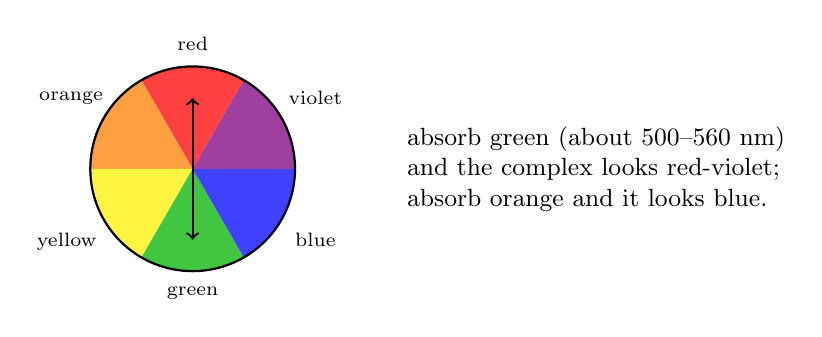
\begin{tikzpicture}[font=\scriptsize]
  \foreach \a/\c/\n in {90/red/red, 150/orange/orange, 210/yellow/yellow, 270/green!70!black/green, 330/blue/blue, 30/violet/violet} {
    \fill[\c!75] (0,0) -- (\a-30:1.3) arc[start angle=\a-30, end angle=\a+30, radius=1.3] -- cycle;
    \node[anchor=\a+180] at (\a:1.38) {\n};
  }
  \draw[thick] (0,0) circle (1.3);
  \draw[<->, thick] (90:0.9) -- (270:0.9);
  \node[anchor=west, font=\small, align=left] at (2.6,0) {absorb green (about 500--560 nm)\\ and the complex looks red-violet;\\ absorb orange and it looks blue.};
\end{tikzpicture}

{\small A colour wheel: the colour seen is roughly the complement, diametrically
opposite, of the band absorbed.}
\end{omfigure}

\begin{definition}[Spectrochemical series]\label{def:b2:ligand-field:spectrochemical}
The \emph{spectrochemical series}\index{spectrochemical series} orders ligands by the
splitting they produce for a given metal ion:
\[
  \ce{I-} < \ce{Br-} < \ce{Cl-} < \ce{F-} < \ce{OH-} < \ce{H2O} < \ce{NH3} < \text{en} <
  \ce{NO2-} < \ce{CN-} < \ce{CO} .
\]
For a given ligand, $\Delta_o$ also grows with the charge of the metal ion and down a group
(4d and 5d complexes, larger than 3d, are almost always \omterm{def:b2:ligand-field:spin}{low spin}).
\end{definition}

The halides are at the weak end and \ce{CN-} and \ce{CO} at the strong end, which the
\omterm{def:b2:ligand-field:crystal-field}{crystal-field model} cannot explain: it would put the charged \ce{F-} above the neutral
\ce{CO}. The explanation needs orbitals.

\section{The ligand field}

\begin{definition}[Ligand field theory]\label{def:b2:ligand-field:ligand-field}
\emph{Ligand field theory}\index{ligand field theory} describes a complex with \omterm{def:b2:diatomic-mos:lcao}{molecular
orbitals} built from the valence orbitals of the metal (its nine $n$d, $(n+1)$s and $(n+1)$p
orbitals) and the donor orbitals of the ligands.
\end{definition}

\begin{proposition}[$\sigma$ bonding in an octahedral complex]\label{prop:b2:ligand-field:mo-octahedral}
With six ligands each giving one $\sigma$ donor orbital, six bonding \omterm{def:b2:diatomic-mos:lcao}{molecular orbitals} form
from the metal's s, three p and the two $e_g$ d orbitals; the three $t_{2g}$ orbitals, which
point between the ligands, stay nonbonding; above them lie the antibonding $e_g^*$
orbitals. The ligand electrons fill the six \omterm{def:b2:diatomic-mos:bonding}{bonding orbitals}; the metal's d electrons go
into $t_{2g}$ and $e_g^*$, separated by $\Delta_o$. Bonding plus \omterm{def:b2:diatomic-mos:bonding}{nonbonding orbitals} can hold
$12 + 6 = 18$ electrons.
\end{proposition}

\begin{proof}[Argument]
By the fragment method of \cref{ch:b2:fragment-orbitals}, each metal orbital interacts
with the combination of ligand orbitals of the same symmetry: s with the totally
symmetric one, each p with a pair of opposite ligands, $\mathrm d_{z^2}$ and $\mathrm
d_{x^2-y^2}$ with the combinations pointing along their lobes; no $\sigma$ combination
matches the $t_{2g}$ orbitals (their overlap with any $\sigma$ donor pointing along an axis
is zero by symmetry). The names of the combinations come from group theory, admitted.
Filling all the bonding and \omterm{def:b2:diatomic-mos:bonding}{nonbonding orbitals}, and none of the antibonding ones, takes
18 electrons --- the \omterm{def:b2:coordination-complexes:electron-count}{18-electron rule}.
\end{proof}

\begin{omfigure}
\begin{tikzpicture}[font=\scriptsize]
  % metal
  \pic (m4p1) at (-0.45,2.6) {omlevel={empty}{0.4}}; \pic (m4p2) at (0,2.6) {omlevel={empty}{0.4}}; \pic (m4p3) at (0.45,2.6) {omlevel={empty}{0.4}};
  \node[anchor=east] at (-0.7,2.6) {$(n{+}1)$p};
  \pic (m4s) at (0,1.8) {omlevel={empty}{0.6}}; \node[anchor=east] at (-0.35,1.8) {$(n{+}1)$s};
  \foreach \x in {-0.9,-0.45,0,0.45,0.9} \pic at (\x,0.6) {omlevel={empty}{0.4}};
  \coordinate (m3d) at (1.1,0.6); \node[anchor=east] at (-1.15,0.6) {$n$d};
  \node[font=\small] at (0,-2.9) {metal};
  % ligands
  \foreach \x in {6.2,6.72,7.24,7.76,8.28,8.8} \pic at (\x,-0.9) {omlevel={ud}{0.36}};
  \coordinate (lig) at (6.0,-0.9);
  \node[font=\small] at (7.3,-2.9) {six $\sigma$ donor orbitals};
  % MOs
  \pic (b1) at (3.6,-2.4) {omlevel={ud}{0.5}};
  \foreach \x in {3.0,3.6,4.2} \pic at (\x,-1.9) {omlevel={ud}{0.5}};
  \pic at (3.3,-1.45) {omlevel={ud}{0.5}}; \pic at (3.9,-1.45) {omlevel={ud}{0.5}};
  \foreach \x in {3.0,3.6,4.2} \pic at (\x,0.3) {omlevel={empty}{0.5}};
  \pic at (3.3,1.5) {omlevel={empty}{0.5}}; \pic at (3.9,1.5) {omlevel={empty}{0.5}};
  \pic at (3.6,3.1) {omlevel={empty}{0.5}};
  \foreach \x in {3.0,3.6,4.2} \pic at (\x,3.6) {omlevel={empty}{0.5}};
  \node[anchor=north] at (3.6,0.12) {$t_{2g}$ (nonbonding)};
  \node[anchor=west] at (4.2,1.5) {$e_g^*$};
  \node[anchor=north] at (3.6,-2.58) {6 bonding};
  \draw[<->, omProp] (2.55,0.3) -- (2.55,1.5) node[midway, right] {$\Delta_o$};
  \draw[omcorr, densely dashed] (m3d) -- (2.75,0.3) (m3d) -- (3.05,1.5) (1.1,0.6) -- (3.05,-1.45);
  \draw[omcorr, densely dashed] (lig) -- (4.15,-1.45) (lig) -- (4.45,-1.9) (lig) -- (3.85,-2.4) (lig) -- (4.15,1.5);
  \draw[omcorr, densely dashed] (m4s-r) -- (3.35,-2.4) (m4s-r) -- (3.35,3.1) (m4p3-r) -- (2.75,-1.9) (m4p3-r) -- (2.75,3.6);
\end{tikzpicture}

{\small \omterm{def:b2:diatomic-mos:lcao}{Molecular orbitals} of an octahedral complex with six $\sigma$ donors,
schematic. The ligands' twelve electrons fill the six \omterm{def:b2:diatomic-mos:bonding}{bonding orbitals}; the metal's d
electrons occupy the nonbonding $t_{2g}$ and the antibonding $e_g^*$ levels, separated by
$\Delta_o$ --- the crystal-field picture recovered. Up to 18 electrons fill the bonding and
nonbonding levels.}
\end{omfigure}

\begin{definition}[$\pi$-donor and $\pi$-acceptor ligands]\label{def:b2:ligand-field:pi-ligands}
A \emph{$\pi$-donor ligand}\index{pi-donor ligand@$\pi$-donor ligand} has filled orbitals
of $\pi$ symmetry with respect to the metal--ligand bond (lone pairs of \ce{Cl-},
\ce{OH-}); a \emph{$\pi$-acceptor ligand}\index{pi-acceptor ligand@$\pi$-acceptor ligand}
has empty ones of low energy (the $\pi^*$ orbitals of \ce{CO} and \ce{CN-}). The transfer of
electron density from filled metal d orbitals into the empty $\pi^*$ orbitals of a
$\pi$-acceptor ligand is called \emph{back-donation}\index{back-donation}.
\end{definition}

\begin{proposition}[$\pi$ effects on the splitting]\label{prop:b2:ligand-field:pi-effects}
$\pi$-donor ligands decrease $\Delta_o$; $\pi$-acceptor ligands increase it.
\end{proposition}

\begin{proof}
The $t_{2g}$ orbitals have the right symmetry to overlap with ligand $\pi$ orbitals. A filled
ligand $\pi$ orbital lies below $t_{2g}$: by \cref{thm:b2:frontier-orbitals:perturbation} the
interaction pushes $t_{2g}$ up, towards $e_g^*$, and $\Delta_o$ shrinks. An empty $\pi^*$ orbital
lies above $t_{2g}$: the interaction pushes $t_{2g}$ down, and $\Delta_o$ grows. The second case
transfers metal d density into the ligand's $\pi^*$: \omterm{def:b2:ligand-field:pi-ligands}{back-donation}.
\end{proof}

\begin{omfigure}
\begin{tikzpicture}[font=\scriptsize]
  \begin{scope}
    \pic (t) at (0,1.2) {omlevel={empty}{0.6}}; \node[anchor=east] at (-0.35,1.2) {$t_{2g}$};
    \pic (l) at (2.4,0) {omlevel={ud}{0.6}}; \node[anchor=west] at (2.75,0) {ligand $\pi$ (filled)};
    \pic (n) at (1.2,1.75) {omlevel={empty}{0.6}};
    \draw[omcorr, densely dashed] (t-r) -- (n-l) (l-l) -- (n-r);
    \pic (e) at (1.2,3.0) {omlevel={empty}{0.6}}; \node[anchor=west] at (1.55,3.0) {$e_g^*$};
    \draw[<->, omProp] (0.55,1.75) -- (0.55,3.0) node[midway, left] {$\Delta_o$ smaller};
    \node[font=\small] at (1.2,-0.8) {$\pi$ donor};
  \end{scope}
  \begin{scope}[xshift=6.5cm]
    \pic (t) at (0,1.2) {omlevel={empty}{0.6}}; \node[anchor=east] at (-0.35,1.2) {$t_{2g}$};
    \pic (l) at (2.4,2.6) {omlevel={empty}{0.6}}; \node[anchor=west] at (2.75,2.6) {ligand $\pi^*$ (empty)};
    \pic (n) at (1.2,0.65) {omlevel={empty}{0.6}};
    \draw[omcorr, densely dashed] (t-r) -- (n-l) (l-l) -- (n-r);
    \pic (e) at (1.2,3.0) {omlevel={empty}{0.6}}; \node[anchor=west] at (1.55,3.15) {$e_g^*$};
    \draw[<->, omProp] (0.55,0.65) -- (0.55,3.0) node[midway, left] {$\Delta_o$ larger};
    \node[font=\small] at (1.2,-0.8) {$\pi$ acceptor (back-donation)};
  \end{scope}
\end{tikzpicture}

{\small Effect of ligand $\pi$ orbitals on the $t_{2g}$ level, schematic. A filled ligand $\pi$
orbital below pushes $t_{2g}$ up (smaller splitting); an empty $\pi^*$ orbital above pulls it
down (larger splitting).}
\end{omfigure}

This places \ce{CO} and \ce{CN-}, strong $\sigma$ donors and $\pi$ acceptors, at the top of the
\omterm{def:b2:ligand-field:spectrochemical}{spectrochemical series}, and the halides, $\pi$ donors, at the bottom. Metal carbonyls have
their $t_{2g}$ orbitals stabilised and filled: the 18-electron complexes of
\cref{ch:b2:coordination-complexes}.

\section{Exercises}

\begin{exercise}[$\star$]\label{exo:b2:ligand-field:1}
Give the octahedral configuration and CFSE of a $d^3$ ion and of a $d^8$ ion.
\end{exercise}

\begin{exercise}[$\star$]\label{exo:b2:ligand-field:2}
How many unpaired electrons do \ce{[Fe(H2O)6]^2+} (\omterm{def:b2:ligand-field:spin}{high spin}) and \ce{[Fe(CN)6]^4-} (\omterm{def:b2:ligand-field:spin}{low
spin}) have?
\end{exercise}

\begin{exercise}[$\star$]\label{exo:b2:ligand-field:3}
A complex absorbs most strongly at \qty{600}{nm}. What colour does it look?
\end{exercise}

\begin{exercise}[$\star$]\label{exo:b2:ligand-field:4}
Order \ce{H2O}, \ce{CN-}, \ce{Cl-}, \ce{NH3} by the splitting they produce.
\end{exercise}

\begin{exercise}[$\star\star$]\label{exo:b2:ligand-field:5}
For a $d^5$ ion, $\Delta_o = \qty{165}{kJ/mol}$ with water and $\qty{390}{kJ/mol}$ with cyanide,
and $P = \qty{300}{kJ/mol}$ (exercise data). Predict both spin states and the unpaired
electrons.
\end{exercise}

\begin{exercise}[$\star\star$]\label{exo:b2:ligand-field:6}
\ce{[Co(H2O)6]^2+} is pink, \ce{[CoCl4]^2-} deep blue. Explain the change of colour from the
change of geometry and ligand.
\end{exercise}

\begin{exercise}[$\star\star$]\label{exo:b2:ligand-field:7}
Show that square-planar \ce{[Ni(CN)4]^2-} is \omterm{def:b2:diatomic-mos:magnetism}{diamagnetic}, while tetrahedral
\ce{[NiCl4]^2-} has two unpaired electrons.
\end{exercise}

\begin{exercise}[$\star\star$]\label{exo:b2:ligand-field:8}
A $d^1$ complex absorbs at \qty{500}{nm} (exercise data). Compute $\Delta_o$ in \unit{cm^{-1}} and
\unit{kJ/mol}.
\end{exercise}

\begin{exercise}[$\star\star$]\label{exo:b2:ligand-field:9}
Why are compounds of \ce{Zn^2+} and \ce{Sc^3+} colourless?
\end{exercise}

\begin{exercise}[$\star\star\star$]\label{exo:b2:ligand-field:10}
Count the electrons in the \omterm{def:b2:diatomic-mos:lcao}{molecular orbitals} of \ce{[Co(NH3)6]^3+}: which levels are filled,
and is the complex \omterm{def:b2:diatomic-mos:magnetism}{diamagnetic}?
\end{exercise}

\begin{exercise}[$\star\star\star$]\label{exo:b2:ligand-field:11}
Explain why \ce{CO}, a neutral and weakly basic molecule, produces a larger splitting than
the fluoride ion.
\end{exercise}

\begin{exercise}[$\star\star\star$]\label{exo:b2:ligand-field:12}
The hydration enthalpies of the \ce{M^2+} ions from \ce{Ca^2+} to \ce{Zn^2+}, plotted against $n$, form
two humps above a straight line through $d^0$, $d^5$ and $d^{10}$. Explain the shape with the
high-spin CFSE.
\end{exercise}

\section{Problem: Red Ruby, Green Emerald}

\begin{problem}[{Weekend problem --- chromium(III) in an octahedral field, the absorption
bands of ruby and the colour they leave, the weaker field of emerald, and hydrated and
anhydrous copper sulfate}]
\label{pb:b2:ligand-field:1}
Data stated for the problem (rounded, illustrative): ruby (\ce{Cr^3+} in \ce{Al2O3}) absorbs
in two bands, near \qty{556}{nm} and \qty{405}{nm}; in emerald (\ce{Cr^3+} in beryl) the
first band lies near \qty{620}{nm}. For a $d^3$ ion the first band corresponds to
$\Delta_o$. $N_Ahc = \qty{0.1196}{J.m/mol}$.
% ledger: const:NA, const:h, const:c

\medskip
\noindent\textbf{Part I --- Chromium(III).}
\begin{enumerate}
  \item Give the $d^n$ configuration of \ce{Cr^3+}.
  \item How is it distributed in an octahedral field?
  \item Is there a choice between high and \omterm{def:b2:ligand-field:spin}{low spin}?
  \item Compute its CFSE.
  \item How many unpaired electrons does it have?
  \item Why are chromium(III) complexes kinetically inert (slow to exchange ligands)?
\end{enumerate}

\medskip
\noindent\textbf{Part II --- Ruby.}
\begin{enumerate}[resume]
  \item What surrounds a \ce{Cr^3+} ion substituted for \ce{Al^3+} in corundum?
  \item Convert the first band to wavenumber.
  \item Deduce $\Delta_o$ in \unit{kJ/mol}.
  \item Which colours are absorbed by the two bands?
  \item What remains to be seen?
  \item Why are there two bands for a single splitting? (A qualitative answer.)
\end{enumerate}

\medskip
\noindent\textbf{Part III --- Emerald.}
\begin{enumerate}[resume]
  \item Convert the emerald band to $\Delta_o$.
  \item Compare with ruby: which crystal gives the stronger field?
  \item Where does the absorbed colour move, and what colour is transmitted?
  \item Suggest a structural reason for the weaker field in beryl.
  \item Would the number of unpaired electrons change?
\end{enumerate}

\medskip
\noindent\textbf{Part IV --- Copper sulfate.}
\begin{enumerate}[resume]
  \item What is the configuration of \ce{Cu^2+}?
  \item In \ce{CuSO4.5H2O}, copper is surrounded by water molecules. Why is the solid blue?
  \item What happens to the colour when the water is driven off, and why?
  \item Why does a drop of water turn the white powder blue again?
  \item Would \ce{[Cu(NH3)4]^2+} absorb at shorter or longer wavelength than the aqua ion?
  \item Can a $d^9$ ion be high or \omterm{def:b2:ligand-field:spin}{low spin}?
  \item Is \ce{CuSO4.5H2O} \omterm{def:b2:diatomic-mos:magnetism}{paramagnetic}?
  \item State $\Delta_o$ of \ce{Cr^3+} in ruby from its first absorption band.
\end{enumerate}
\end{problem}
